\documentclass[man,floatsintext]{apa6}
\usepackage{lmodern}
\usepackage{amssymb,amsmath}
\usepackage{ifxetex,ifluatex}
\usepackage{fixltx2e} % provides \textsubscript
\ifnum 0\ifxetex 1\fi\ifluatex 1\fi=0 % if pdftex
  \usepackage[T1]{fontenc}
  \usepackage[utf8]{inputenc}
\else % if luatex or xelatex
  \ifxetex
    \usepackage{mathspec}
  \else
    \usepackage{fontspec}
  \fi
  \defaultfontfeatures{Ligatures=TeX,Scale=MatchLowercase}
\fi
% use upquote if available, for straight quotes in verbatim environments
\IfFileExists{upquote.sty}{\usepackage{upquote}}{}
% use microtype if available
\IfFileExists{microtype.sty}{%
\usepackage{microtype}
\UseMicrotypeSet[protrusion]{basicmath} % disable protrusion for tt fonts
}{}
\usepackage{hyperref}
\hypersetup{unicode=true,
            pdftitle={What's she talking about? Category based discourse inferences in early childhood},
            pdfauthor={Manuel Bohn, Khuyen Nha Le, Benjamin Peloquin, Bahar Köymen, \& Michael C. Frank},
            pdfkeywords={keywords},
            pdfborder={0 0 0},
            breaklinks=true}
\urlstyle{same}  % don't use monospace font for urls
\usepackage{graphicx,grffile}
\makeatletter
\def\maxwidth{\ifdim\Gin@nat@width>\linewidth\linewidth\else\Gin@nat@width\fi}
\def\maxheight{\ifdim\Gin@nat@height>\textheight\textheight\else\Gin@nat@height\fi}
\makeatother
% Scale images if necessary, so that they will not overflow the page
% margins by default, and it is still possible to overwrite the defaults
% using explicit options in \includegraphics[width, height, ...]{}
\setkeys{Gin}{width=\maxwidth,height=\maxheight,keepaspectratio}
\IfFileExists{parskip.sty}{%
\usepackage{parskip}
}{% else
\setlength{\parindent}{0pt}
\setlength{\parskip}{6pt plus 2pt minus 1pt}
}
\setlength{\emergencystretch}{3em}  % prevent overfull lines
\providecommand{\tightlist}{%
  \setlength{\itemsep}{0pt}\setlength{\parskip}{0pt}}
\setcounter{secnumdepth}{0}
% Redefines (sub)paragraphs to behave more like sections
\ifx\paragraph\undefined\else
\let\oldparagraph\paragraph
\renewcommand{\paragraph}[1]{\oldparagraph{#1}\mbox{}}
\fi
\ifx\subparagraph\undefined\else
\let\oldsubparagraph\subparagraph
\renewcommand{\subparagraph}[1]{\oldsubparagraph{#1}\mbox{}}
\fi

%%% Use protect on footnotes to avoid problems with footnotes in titles
\let\rmarkdownfootnote\footnote%
\def\footnote{\protect\rmarkdownfootnote}


  \title{What's she talking about? Category based discourse inferences in early
childhood}
    \author{Manuel Bohn\textsuperscript{1,2}, Khuyen Nha Le\textsuperscript{1},
Benjamin Peloquin\textsuperscript{1}, Bahar Köymen\textsuperscript{3},
\& Michael C. Frank\textsuperscript{1}}
    \date{}
  
\shorttitle{Discourse inferences in early childhood}
\affiliation{
\vspace{0.5cm}
\textsuperscript{1} Stanford University\\\textsuperscript{2} Leipzig University\\\textsuperscript{3} University of Manchester}
\keywords{keywords\newline\indent Word count: X}
\usepackage{csquotes}
\usepackage{upgreek}
\captionsetup{font=singlespacing,justification=justified}

\usepackage{longtable}
\usepackage{lscape}
\usepackage{multirow}
\usepackage{tabularx}
\usepackage[flushleft]{threeparttable}
\usepackage{threeparttablex}

\newenvironment{lltable}{\begin{landscape}\begin{center}\begin{ThreePartTable}}{\end{ThreePartTable}\end{center}\end{landscape}}

\makeatletter
\newcommand\LastLTentrywidth{1em}
\newlength\longtablewidth
\setlength{\longtablewidth}{1in}
\newcommand{\getlongtablewidth}{\begingroup \ifcsname LT@\roman{LT@tables}\endcsname \global\longtablewidth=0pt \renewcommand{\LT@entry}[2]{\global\advance\longtablewidth by ##2\relax\gdef\LastLTentrywidth{##2}}\@nameuse{LT@\roman{LT@tables}} \fi \endgroup}


\usepackage{lineno}

\linenumbers

\authornote{We thank Megan Merrick and Sabina Zacco for their
help with the data collection. MB received funding from the European
Union's Horizon 2020 research and innovation programme under the Marie
Sklodowska-Curie grant agreement no. 749229.

Correspondence concerning this article should be addressed to Manuel
Bohn, Jahnallee 59, 04109 Leipzig, Germany. E-mail:
\href{mailto:manuel.bohn@uni-leipzig.de}{\nolinkurl{manuel.bohn@uni-leipzig.de}}}

\abstract{
tbd\ldots{}


}

\begin{document}
\maketitle

\section{Experiment 1}\label{experiment-1}

All experimental procedures, sample sizes and statistical analysis were
pre-registered (see \url{https://osf.io/9ypxn} and
\url{https://osf.io/fyaxq}). The experimental procedure can be found in
the assoicated online repository at
\url{https://github.com/manuelbohn/disCon}.

\subsection{Participants}\label{participants}

We obtained valid data from 71 children, including 30 2-year-olds (mean
= 2.63, range = 2.00 - 2.98), 21 3-year-olds (mean = 3.56, range = 3.13
- 3.97) and 20 4-year-olds (mean = 4.50, range = 4.00 - 4.97). We tested
a larger sample of 2-year-olds because we expected a weaker effect in
this age group. In addition, 12 children were recruited but not tested
becasue their parents reported less than 75\% of English exposure at
home. Ten children started the experiment but did not finish it because
they became impatient (7) or the equipment broke (3). Three children
were tested but excluded becasue they were correct in less than 5/6
training trials (see below). All children were recruited from the floor
of a Children's museum in San José, California, USA. The population from
which this sample is drawn is characterised by diverse ethnic background
and high socioeconimic status. Parents gave informed consent and
provided demographic information. All experiments reported in this paper
were approved by the Stanford Institutional Review Board (protocol no.
357 19960).

\begin{figure}

{\centering 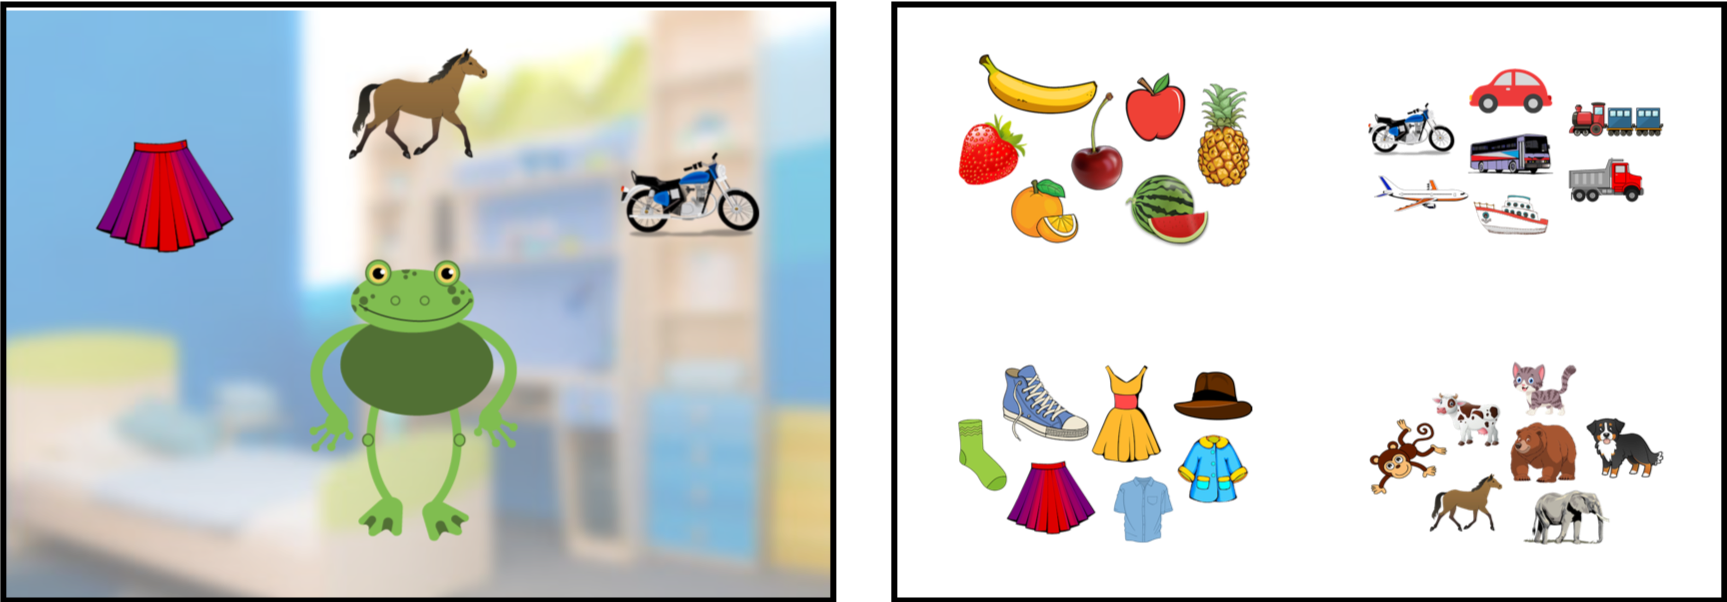
\includegraphics[width=450px]{../figures/setup} 

}

\caption{Left: Screenshot from the experimental setup. Right: Stimuli pictures for the four categories: fruits, vehicles, clothes and mammals.}\label{fig:fig1}
\end{figure}

\subsection{Method}\label{method}

Study materials were presented as a picture book on a tablet computer
(Frank, Sugarman, Horowitz, Lewis, \& Yurovsky, 2016). Children reponded
by touching objects on the screen. Responses were automatically saved.
The experimenter guided children through the procedure and read out
general instructions. The study was framed as visit to the house of the
little animals which would show the child the things they have at home.
Utterances made by the different animals were pre-recorded from native
English speakers, with one speaker per animal. On each trial, children
saw one animal in the middle of the screen with three objects above them
(Figure \ref{fig:fig1}, left). Each objects was from different category
(mammals, vehicles, clothes and fruits). For each category, we had
pictures of seven different category memebers (e.g.~for vehicles: car,
truck, train, bus, airplane, boat and motorbike, see Figure
\ref{fig:fig1}, right). The trial started with six training rounds, in
which the animal named one of the objects above them, asking the child
to touch it (e.g. \enquote{Look at that, can you touch the horse}). From
one round to the next, the pictures changed but the categories remained
the same. For example, children saw a skirt, a horse and a motorcylce on
the first training round and a jacket, a dog and a bus on the second.
During training, the speaker consitently named objects from the same
target category. After six training rounds, children received a test
round in which the speaker used a pronoun to refer to one of the objects
(\enquote{Look at that, can you touch \emph{it}}). Categories were
ranomdly selected at the beginning of each trial and so was the order of
pictures within each category. The position of each picture (left, right
mddle) was also randomly determined on each round. Children received
four trials, one with each category as the target.

\subsection{Results}\label{results}

\begin{figure}

{\centering \includegraphics{manuscript_files/figure-latex/fig2-1} 

}

\caption{A: Posterior probability distribution for the mean for each age bin. Shaded regions indicate 95\% CIs. B: Correct  responses for age continously. Transparent dots show aggregated data from individual participants. Red line with grey shows the smoothed conditional mean of the data in each condition..}\label{fig:fig2}
\end{figure}

The dependent variable in all analysis was whether the touched object at
test was from the same category as the objects named throughout the
training rounds. All following analysis were computed in R (R Core Team,
2018). As a first step, we aggregated respones across trials for each
child and compared the proportion of correct responses to a level
expected by chance (33\% correct) within each age bin. We used the
function \texttt{ttestBF} from the R-package \texttt{BayesFactor} (Morey
\& Rouder, 2018) to compute a Bayes factor (BF) in favor of the
hypothesis that performance is above chance (see Figure
\ref{fig:fig2}A). We found little evidence that 2-year olds performed
above chance (mean proportion correct = 0.42, BF = 0.59) but found
subtantial evidence for 3-year-olds (mean proportion correct = 0.60, BF
= 90.77) and 4-year-olds (mean proportion correct = 0.55, BF = 10.39).

To analyse responses continously across age we used generalized linear
mixed models (GLMM) fit via the function \texttt{brm} from the R-package
\texttt{brms} (Bürkner, 2017). All models had default priors and
included random effects for participant id and speaker. Inference was
based on comparing models that differed in whether they included the key
predictor of interest, in this case age. Following McElreath (2016), we
compared models using WAIC (widely applicable information criterion)
scores and weights. WAIC is an indicator of the model's predictive
accuracy for out of sample data and model's with lower scores are
preferred. WAIC weights are an estimate of the probability that this
model (compared to all other models considered) will make the best
predictions on new data. We quantified the evidence in favor of the
model with the lowest WAIC score (highest WAIC weight) compared to
alternative models by computing Bayes factors via the funtion
\texttt{bayes\_factor} from the R-package \texttt{brms} (Bürkner, 2017).

The model comparison favored the model including age as a predictor
(Table \ref{tab:table1}). The model estiamte for age was positive
(\(\beta\) = 0.32, 95\% confidence interval (CI) = -0.08 - 0.75),
suggesting an increase in performance with age (see also Figure
\ref{fig:fig2}B). However, the evidence in support of this model was
modest, speaking against subtantial developmental gains across the age
range considered.

\subsection{Discussion}\label{discussion}

\begin{table}[tbp]
\begin{center}
\begin{threeparttable}
\caption{\label{tab:table1}Model comparison for Experiment 1}
\begin{tabular}{lllll}
\toprule
Model & \multicolumn{1}{c}{WAIC} & \multicolumn{1}{c}{SE} & \multicolumn{1}{c}{weight} & \multicolumn{1}{c}{BF}\\
\midrule
correct \textasciitilde{} age + RE & 387.20 & 7.67 & 0.56 & -\\
correct \textasciitilde{} 1 + RE & 387.69 & 7.11 & 0.44 & 1.77\\
\bottomrule
\addlinespace
\end{tabular}
\begin{tablenotes}[para]
\normalsize{\textit{Note.} All models had the same random effects (RE) structure. BF denotes the Bayes Factor in favor to the model with the highest WAIC weight.}
\end{tablenotes}
\end{threeparttable}
\end{center}
\end{table}

\section{Experiment 2}\label{experiment-2}

Registration: \url{https://osf.io/x2k4p}

\subsection{Participants}\label{participants-1}

\subsection{Material and Procedure}\label{material-and-procedure}

\subsection{Results and Discussion}\label{results-and-discussion}

\begin{table}[tbp]
\begin{center}
\begin{threeparttable}
\caption{\label{tab:table2}Model comparison for Experiment 2}
\begin{tabular}{lllll}
\toprule
Model & \multicolumn{1}{c}{WAIC} & \multicolumn{1}{c}{SE} & \multicolumn{1}{c}{weight} & \multicolumn{1}{c}{BF}\\
\midrule
correct \textasciitilde{} age + RE & 176.48 & 9.28 & 0.43 & -\\
correct \textasciitilde{} age * condition + RE & 177.29 & 11.00 & 0.29 & 0.09\\
correct \textasciitilde{} age + condition + RE & 177.36 & 9.93 & 0.28 & 0.45\\
\bottomrule
\addlinespace
\end{tabular}
\begin{tablenotes}[para]
\normalsize{\textit{Note.} All models had the same random effects (RE) structure. BF denotes the Bayes Factor in favor to the model with the highest WAIC weight.}
\end{tablenotes}
\end{threeparttable}
\end{center}
\end{table}

\section{Experiment 3}\label{experiment-3}

Registration: \url{https://osf.io/5e9pk}

\subsection{Participants}\label{participants-2}

\subsection{Material and Procedure}\label{material-and-procedure-1}

\subsection{Results and Discussion}\label{results-and-discussion-1}

\begin{table}[tbp]
\begin{center}
\begin{threeparttable}
\caption{\label{tab:table3}Model comparison for Experiment 3}
\begin{tabular}{lllll}
\toprule
Model & \multicolumn{1}{c}{WAIC} & \multicolumn{1}{c}{SE} & \multicolumn{1}{c}{weight} & \multicolumn{1}{c}{BF}\\
\midrule
correct \textasciitilde{} age * condition + RE & 325.21 & 10.50 & 0.58 & -\\
correct \textasciitilde{} age + condition + RE & 327.25 & 9.52 & 0.21 & 23.91\\
correct \textasciitilde{} age + RE & 327.30 & 8.96 & 0.21 & 23.88\\
\bottomrule
\addlinespace
\end{tabular}
\begin{tablenotes}[para]
\normalsize{\textit{Note.} All models had the same random effects (RE) structure. BF denotes the Bayes Factor in favor to the model with the highest WAIC weight.}
\end{tablenotes}
\end{threeparttable}
\end{center}
\end{table}

\section{General Discussion}\label{general-discussion}

\begin{figure}
\centering
\includegraphics{manuscript_files/figure-latex/plot2-1.pdf}
\caption{}
\end{figure}

\newpage

\section{References}\label{references}

\begingroup
\setlength{\parindent}{-0.5in} \setlength{\leftskip}{0.5in}

\hypertarget{refs}{}
\hypertarget{ref-R-brms_a}{}
Bürkner, P.-C. (2017). brms: An R package for Bayesian multilevel models
using Stan. \emph{Journal of Statistical Software}, \emph{80}(1), 1--28.
doi:\href{https://doi.org/10.18637/jss.v080.i01}{10.18637/jss.v080.i01}

\hypertarget{ref-frank2016using}{}
Frank, M. C., Sugarman, E., Horowitz, A. C., Lewis, M. L., \& Yurovsky,
D. (2016). Using tablets to collect data from young children.
\emph{Journal of Cognition and Development}, \emph{17}(1), 1--17.

\hypertarget{ref-rethinking}{}
McElreath, R. (2016). \emph{Statistical rethinking: A bayesian course
with examples in R and Stan} (pp. xvii, 469). Boca Raton: CRC Press.

\hypertarget{ref-R-BayesFactor}{}
Morey, R. D., \& Rouder, J. N. (2018). \emph{BayesFactor: Computation of
bayes factors for common designs}. Retrieved from
\url{https://CRAN.R-project.org/package=BayesFactor}

\hypertarget{ref-R-base}{}
R Core Team. (2018). \emph{R: A language and environment for statistical
computing}. Vienna, Austria: R Foundation for Statistical Computing.

\endgroup


\end{document}
